\documentclass{article}
\usepackage[margin=3cm]{geometry}
\usepackage[utf8]{inputenc}
\usepackage{amsmath}
\usepackage{amssymb}
\usepackage{float}
\usepackage{enumitem}
\usepackage{graphicx}
\usepackage{caption}
\usepackage{subcaption}
\usepackage{eurosym}

\graphicspath{ {Plots/} }


\begin{document}
	\textit{MS-E2134 - Decision making and problem solving}
	\vfill
	{\centering \Huge Assignment 2 \par}
	\vfill
	Christian Segercrantz - 481056 \\
	\par \today
	\pagebreak
	\tableofcontents
	\pagebreak
\section{Simulation}
\subsection{a)}
\begin{figure}[H]
	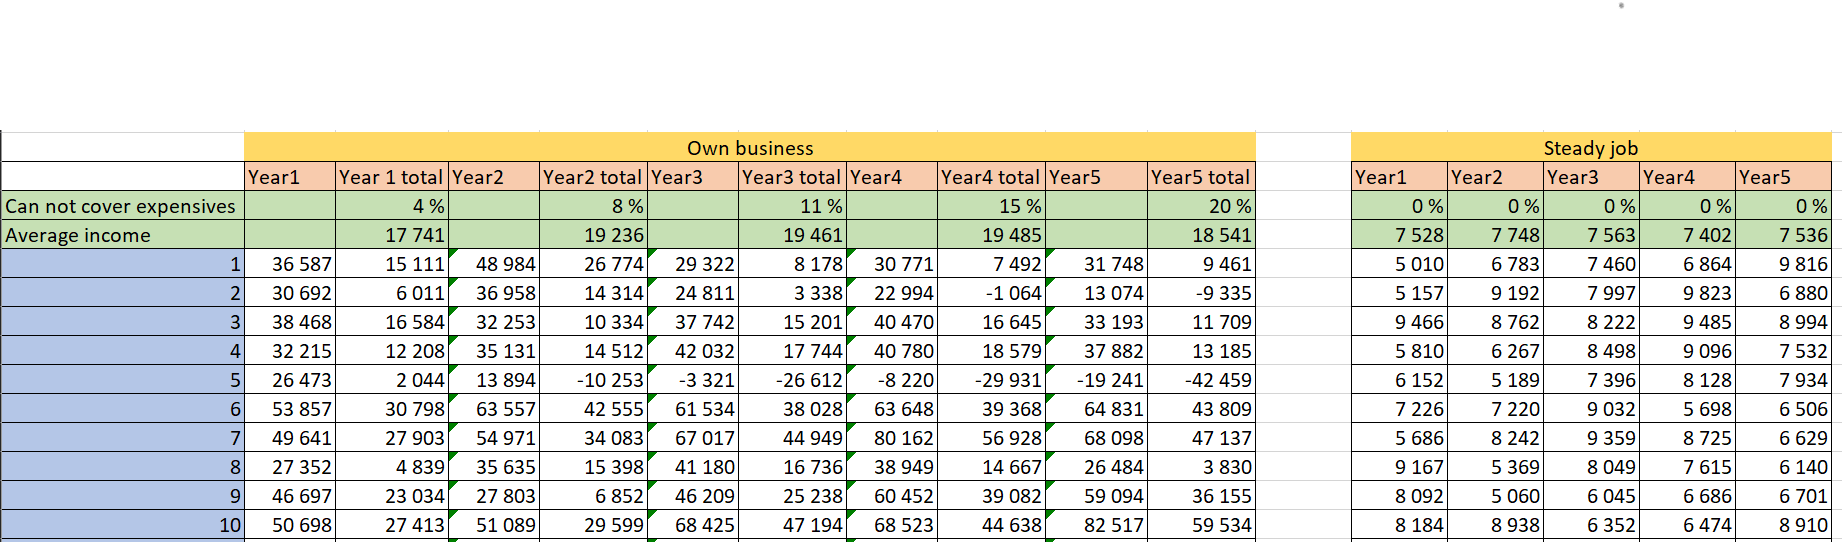
\includegraphics[width=\textwidth]{1a.png}
	\caption{A table displaying ten iterations of the 5 first years for exercise 1.1 a)}
	\label{fig:1a}
\end{figure}

\subsection{b)}

	\begin{table}[h]
		\centering
		\caption{Average cash flow for fives years for both the steady job and own business ventures.}
		\label{tab:1b}
		\begin{tabular}{l|l|l|l|l|l|}
			\cline{2-6}
			& Year 1 & Year 2 & Year 3 & Year 4 & Year 5 \\ \hline
			\multicolumn{1}{|l|}{Steady job}   & 7 528  & 7 748  & 7 563  & 7 402  & 7 536  \\ \hline
			\multicolumn{1}{|l|}{Own business} & 17 741 & 19 236 & 19 461 & 19 485 & 18 541 \\ \hline
		\end{tabular}
	\end{table}
	
	Based on the simulations, it seems that starting the own business venture would for sure be the more lucrative, and better, option. However, an average over 200 replications might give us an overly optimistic outlook.
\subsection{c)}
	We can see the probabilities from Table \ref{tab:1c}. We can see that initially the probability is approximately 5\% and rises to approximately 20\% in year 5. For the steady job, as the maximum of the expenses is less than the constant income, the probability that he is not able to cover his expenses is 0\% for all years.
	\begin{table}[h]
		\centering
		\caption{Probability that Dr. Cuckoo cannot cover his expenses each year for both the steady job and own business ventures.}
		\label{tab:1c}
		\begin{tabular}{l|l|l|l|l|l|}
			\cline{2-6}
			& Year 1 & Year 2 & Year 3 & Year 4 & Year 5 \\ \hline
			\multicolumn{1}{|l|}{Steady job}   & 0 \%   & 0 \%   & 0 \%   & 0 \%   & 0 \%   \\ \hline
			\multicolumn{1}{|l|}{Own business} & 4 \%   & 8 \%   & 11 \%  & 15 \%  & 20 \%  \\ \hline
		\end{tabular}
	\end{table}
\section{Decision trees}
	To make the numbers easier to handle, everything is handled in millions if not otherwise stated.
\subsection{a)}
	The built decision tree can be seen in Figure \ref{fig:2a}. Based on the tree, I should not accept the offer, but instead give a counteroffer.
	\begin{figure}[H]
		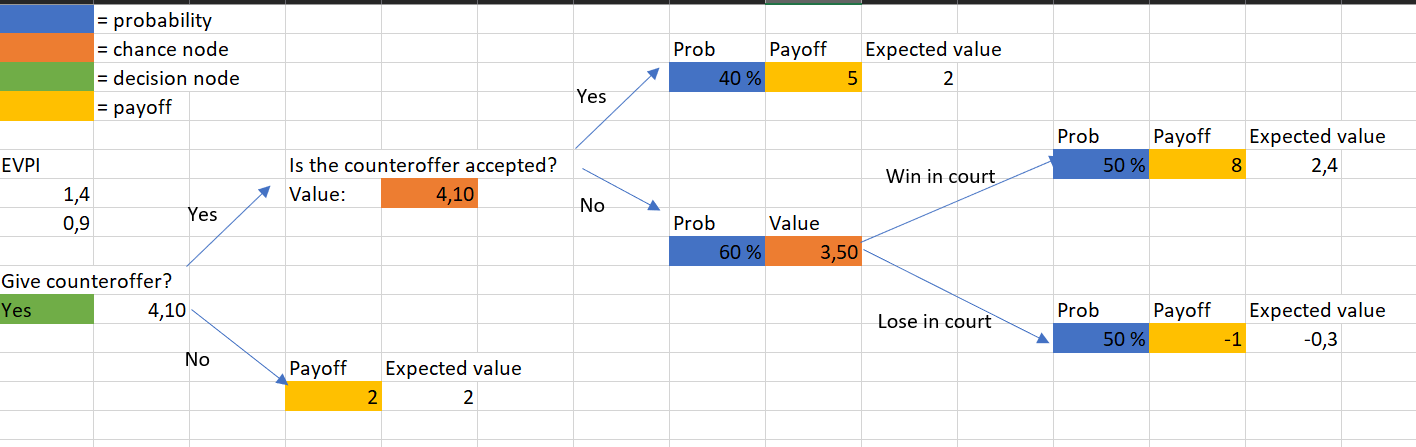
\includegraphics[width=\textwidth]{2a.png}
		\caption{A figure displaying the decision tree 2.2 a)}
		\label{fig:2a}
	\end{figure}
\subsection{b)}
	The value of prefect information (EVPI) can be calculated as the expected value of the possible outcomes times the probability of that outcome minus the expected value of the default decision tree, i.e. $EVPI = EV|PI - EMV$.
	We can build a table for our $EV|PI$-value, it can be seen in Table \ref{tab:2b}.
	\begin{table}[h]
		\centering
		\caption{Table displaying key values of prefect information. }
		\label{tab:2b}
		\begin{tabular}{l|l|l}
			Knowledge                 & Probability & Outcome \\ \hline
			Accept deal + Win court   & 0.2         & 5mil\euro   \\
			Accept deal + Lose court  & 0.2         & 5mil\euro   \\
			Decline deal + Win court  & 0.3         & 8mil\euro   \\
			Decline deal + Lose court & 0.3         & 2mil\euro  
		\end{tabular}
	\end{table}
	The value is thus $EV|PI = 0.2\cdot5+0.2\cdot5+0.3\cdot8+0.3\cdot2 = 5$mil\euro which gives us the result $\text{EVPI} = 5 - 4.1 = 0.9$mil\euro.
\subsection{c)}
	The decision tree for this part can be seen in Figure \ref{fig:2c}. The lower part of the three, where consultation is not chosen, has been replaced by a reference to the original three from part a) which can bee seen in Figure \ref{fig:1a}. All relevant calculations can be seen in the left upper corner of the figure. The complements of $P(W|\text{Pred } W)$ and $P(W|\text{Pred } L)$ has been used directly in the needed probability nodes on the far right. 
	\begin{figure}[H]
		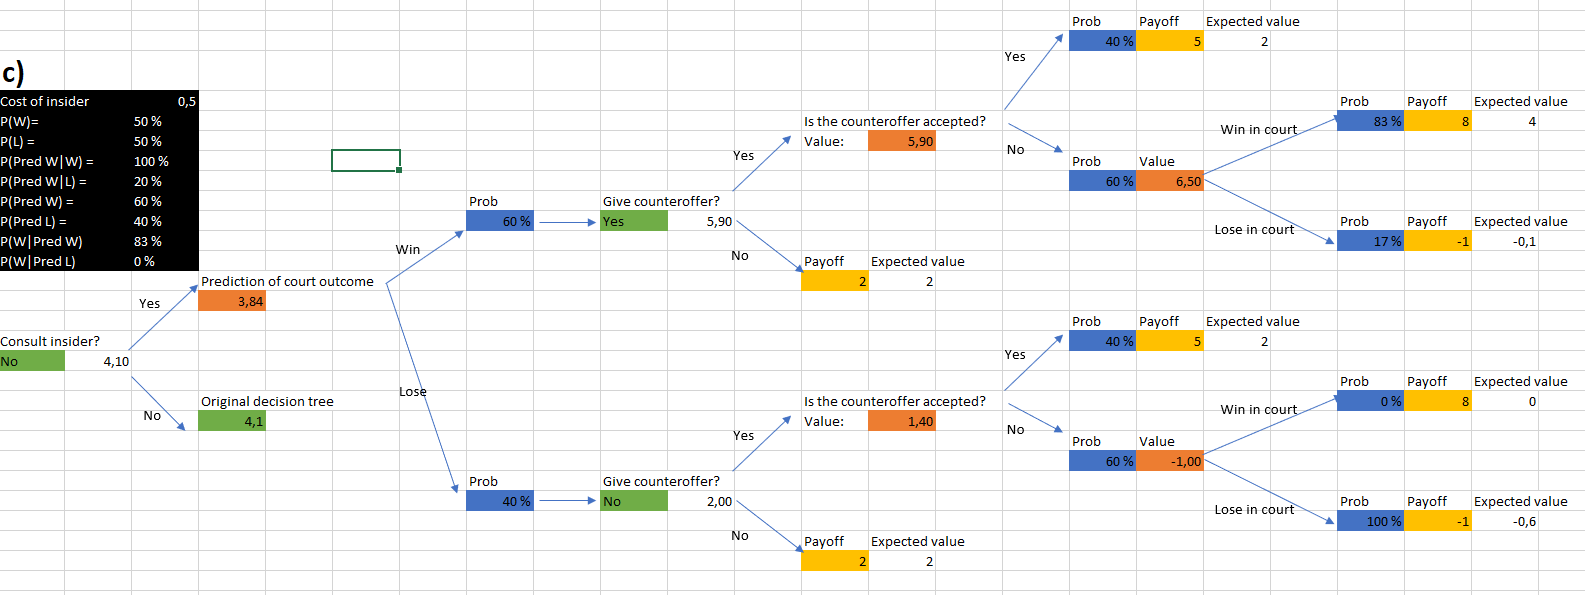
\includegraphics[width=\textwidth]{2c.png}
		\caption{A figure displaying the decision tree 2.2 c)}
		\label{fig:2c}
	\end{figure}
\subsection{d)}
	The optimal sequence of decisions is to not consult the justice system insider, as seen in Figure \ref{fig:2c} and to give a counteroffer, as seen in Figure \ref{fig:2a}.
\subsection{e)}
	The EVSI value can be calculated simply by taking the difference of the branches from the decision of the court insider: $4.1 - 3.84 = 0.24$. This means that we would at most be willing to pay $240$k\euro for the information for it to be worth taking on. In other words, the cost would have to decrease by at least $260$k\euro for us to be interested in it.
	The efficiency can be calculated as $\frac{\text{EVSI}}{\text{EVPI}}*100 = \frac{\text{0.24}}{\text{0.9}}*100 = 26.7\%$.
\subsection{f)}
	In order to calculated the sum we would be willing to pay at maximum to the justice insider we change the probability $P(\text{Pred } W|L) = 0$ i.e. for the insider to have perfect information on the outcome of the court. We can now perform the same calculation as in e) to get the value $300$k\euro for the maximum amount we would be willing to pay.  
\section{Elicitation of utility functions}
	We start by calculating the different values for the utility functions. We normalize the utility function such that $u(10M)=1$ and $u(-2M)=0$. We can thus calculate:
	\begin{align}
		u(1.5\text{M}) &= 0.5u(10\text{M}) + 0.5u(-2\text{M})\\
		u(1.5\text{M}) &= 0.5 \cdot 1 + 0.5 \cdot 0 \\ 
		u(1.5\text{M})&= 0.5 \\
		u(4\text{M}) &= 0.5u(10\text{M}) + 0.5u(1.5\text{M})\\
		u(4\text{M}) &= 0.5 \cdot 1 + 0.5 \cdot 0.5 \\ 
		u(4\text{M})&= 0.75 \\
		u(0.1\text{M}) &= 0.5u(-2\text{M}) + 0.5u(1.5\text{M})\\
		u(0.1\text{M}) &= 0.5 \cdot 0 + 0.5 \cdot 0.5 \\ 
		u(0.1\text{M})&= 0.25 \\
		u(6\text{M}) &= 0.4u(10\text{M}) + 0.6u(4\text{M})\\
		u(6\text{M}) &= 0.4 \cdot 1 + 0.6 \cdot 0.75\\ 
		u(6\text{M})&= 0.85 \\
	\end{align}
	The plotted utility function can be seen in Figure \ref{fig:3}. As we can see, the function is somewhat concave. According to EUT, Dr. Stoveo is, as he says, risk averse.
	\begin{figure}[H]
		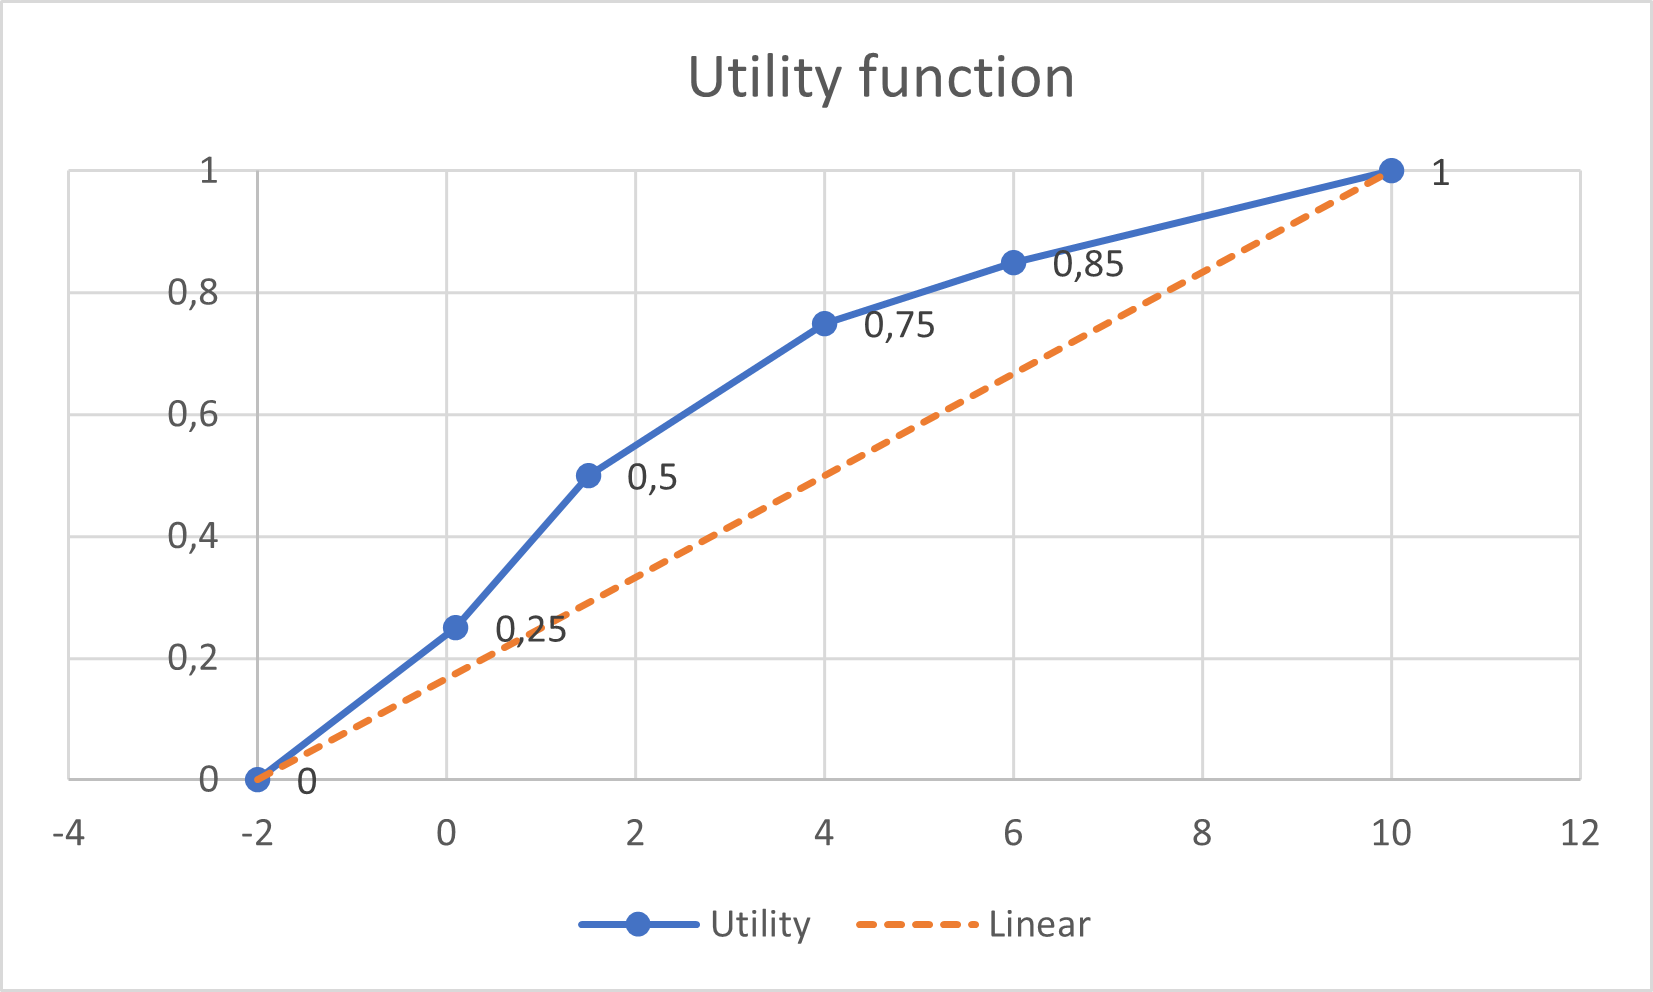
\includegraphics[width=0.9\textwidth]{3.png}
		\caption{The plotted utility function based on Dr. Stoveos choices.}
		\label{fig:3}
	\end{figure}
\section{Expected utility, risk-attitude, and risk measures}
\subsection{a)}
	In order to find out what the investors risk attitude is, we will use first and second order derivatives. 
	\begin{align}
		\frac{d}{dx}\sqrt{x} &= \frac{1}{2}x^{-\frac{1}{2}} \\
		\frac{d^2}{dx^2}\sqrt{x} &= -\frac{1}{4}x^{-\frac{3}{2}} \\
		\frac{d}{dx}x^3 &=  3x^2\\
		\frac{d^2}{dx^2}x^3 &= 6x
	\end{align}
	From these we can see that Rick Averell's utility functions first order derivative is positive for all $x>0$ and hence is the utility function increasing. The second order derivative is negative for all $x>0$ the growth is decreasing. From this we can conclude that the function is concave and Rick Averell is risk averse.
	We can draw conclusions in the same way for Ricki Seeck. Since both order derivatives are positive for all $x>0$, we know that the function is increasingly positive and thus convex. Mr. Seeck's utility function is thus risk seeking. 
\subsection{b)}
\subsubsection{i}
	We can calculate the expected utility as $E[u(X)] = \int f_x(x) u(x)dx$. 
	\begin{equation}
		f_x(t) = 
		\begin{cases}
			 \frac{1}{50}, &  50 \leq x \leq 100 \\
			 0, & \mbox{otherwise}
		\end{cases}
	\end{equation}
	By integrating over the whole space we get,:
	\begin{align}
		\int f_x(x) u(x)dt &= \\
		\int_{50}^{100} \frac{1}{50} u(x) dt& 
	\end{align}
	We count the expected utility for Rick Averell:
	\begin{align}
		\int_{50}^{100} \frac{1}{50} \sqrt{x} dx &=  \\
		\Bigg/_{50}^{100} \frac{1}{50} \frac{3}{2} x^{\frac{3}{2}} = \frac{3}{2} x^{\frac{3}{2}} &= \\
		\Bigg/_{50}^{100} \frac{3}{100} x^{\frac{3}{2}}	& \approx 8.62		
	\end{align}
	Using the same logic we calculate the expected utility for Ricki Seeck:
	\begin{equation}
		\int_{50}^{100} \frac{1}{50} x^3 dx  = 468750.	
	\end{equation}
	To summarize, the expected utilities are $E[u(X)]_{Rick Averall} \approx 8.62$ and $E[u(X)]_{Ricki Seeck} = 468750$
	
	The certainty equivalent is calculated by $CE[x] = u^{-1}(E[u(X)])$. For Rick Averall this means
	\begin{equation}
		CE[x]_{Rick Averall} = u^{-1}(E[u(X)]) = E[u(X)]_{Rick Averall}^2 \approx 74.3
	\end{equation}
	and for Ricki Seeck 
		\begin{equation}
		CE[x]_{Ricki Seeck} = u^{-1}(E[u(X)]) = \sqrt[3]{E[u(X)]_{Ricki Seeck}} \approx 77.7.
	\end{equation}

	The risk premia is calculated as $RP[X] = E[X] - CE[X]$. The expected vlaue is $E(X) = 75$ 
	For Rick Averall this becomes:
	\begin{equation}
		E[X] - CE[x]_{Rick Averall} \approx 0.7,
	\end{equation}
	and for Ricki Seeck:
		\begin{equation}
		E[X] - CE[x]_{Ricki Seeck} \approx -2.7.
	\end{equation}
	Since Rick Averall's risk premia is postivie and Ricki Seeck's is negative, they are inline with our earlier interpretation of the risk attitudes.
\subsubsection{ii}
	The calculations can be seen in the attached .mlx file. The values we received were approximately the following:\\
	$E[u(X)]_{Rick Averall} = 5.1$ \\
	$E[u(X)]_{Ricki Seeck} = 6\cdot10^5$\\
	$CE[x]_{Rick Averall} = 26.3 $ \\
	$CE[x]_{Ricki Seeck} = 84.7$ \\
	$RP[X]_{Rick Averall} = 7.2$ \\
	$RP[X]_{Ricki Seeck} = -51.1$ \\
	These numbers are inline with our conclusions from part a) about the risk attitudes of the DM's.
\subsubsection{iii}
	The calculations can be seen in the attached .mlx file. The values we received were approximately the following:\\
	$E[u(X)]_{Rick Averall} = 9.49$ \\
	$E[u(X)]_{Ricki Seeck} = 1.64\cdot10^6$\\
	$CE[x]_{Rick Averall} = 90.00 $ \\
	$CE[x]_{Ricki Seeck} = 117.83$ \\
	$RP[X]_{Rick Averall} = 8.25$ \\
	$RP[X]_{Ricki Seeck} = -19.58$ \\
	These numbers are inline with our conclusions from part a) about the risk attitudes of the DM's.
\subsection{c)}
\subsubsection{i}
	We start by analytically calculating the $10\%$ Value-at-Risk (VaR) and Conditional Value-at-Risk (CVaR)  for the uniform distribution. The VaR is calculated as 
	\begin{equation}
		\int_{-\infty}^{\text{VaR}_\alpha [X]} f_X(t)dt = \alpha = F_X(\text{VaR}_{\alpha}[X]) \iff \text{VaR}_\alpha [X] =  F_X^{-1}(\alpha).
	\end{equation}
	Let's compute the inverse of the CDF of our function.
	\begin{align}
		F_X &= 
		\begin{cases}
			0 , & x < 50 \\
			 \frac{x-50}{50}, &  50 \leq x \leq 100 \\
			1, & 100 < x
		\end{cases} \\
		\implies F^{-1}_X &= 
			50x + 50,   50 \leq x \leq 100 \\
	\end{align}
	Using this we can the substitute x for $\alpha = 0.1$
	\begin{equation}
		\text{VaR}_{0.1} [X] = F^{-1}_X(0.1) = 55.
	\end{equation}
	We can now calculate the CVar as 
	\begin{equation}
		E[X | X \leq \text{VaR}_\alpha [X]] = \int_{-\infty}^{\text{VaR}_\alpha [X]} x \frac{f_x(x)}{\alpha} dx.
	\end{equation} 
	For our unifrom function this becomes
	\begin{align}
		\text{CVaR}_{10\%} &=  \int_{50}^{55} x \frac{1/50}{0.1} dx \\
		 & = \Bigg/_{50}^{55} \frac{x^2}{10} \\
		 & =  52.5.
	\end{align}
	To summarize $\text{VaR}_{10\%}=55$ and $\text{CVaR}_{10\%}=52.5$.
\subsubsection{ii}
	The calculations can be seen in the attached .mlx file. We receive the values $\text{VaR}_{10\%} = 5.6$ and $\text{CVaR}_{10\%} = 3.6$.
\subsubsection{iii}
	The calculations can be seen in the attached .mlx file. We receive the values $\text{VaR}_{10\%} = 10$ and $\text{CVaR}_{10\%} = 7.50$.
\section{Stochastic dominance}
\subsection{a)}
	From Figure \ref{fig:5} we can see that discrete distribution nearly first order stochastic dominates the Log-normal distribution but since the Log-normal distribution never actually reaches 1 and the discrete distribution does at 200, there is no first order stochastic domination
	
%	From Figure \ref{fig:5} we can see that the discrete distribution first order stochastic dominates the Log-normal distribution since it's always below.
%	\begin{equation}
%		\text{Discrete}  \succcurlyeq_{FSD} \text{LogN}(3,1^2)
%	\end{equation}
	\begin{figure}[H]
		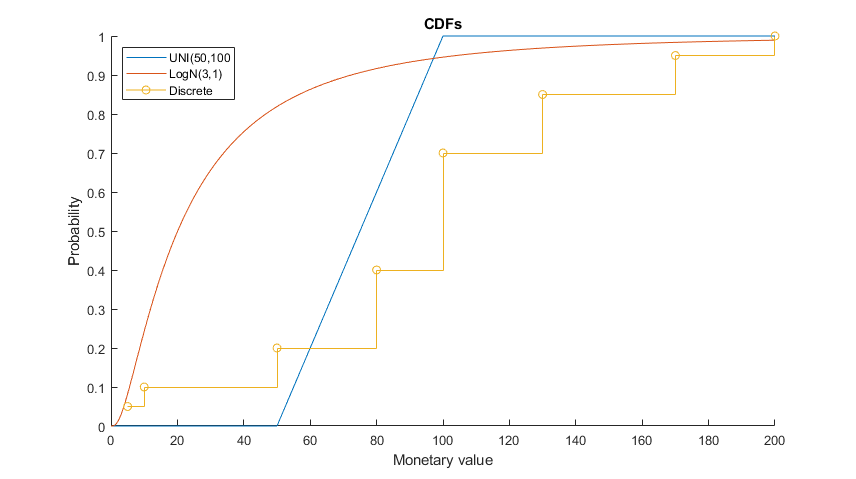
\includegraphics[width=0.8\textwidth]{5.png}
		\caption{The cumulative distribution functions for the three distributions.}
		\label{fig:5}
	\end{figure}
\subsection{b)}
	We can identify three different second order stochastic dominations from the CDF's
	\begin{enumerate}
		\item The discretre distribution dominates the Log-normal distrubtion as a result of it's nearly first order stochastic dominance.
		\item By examining the plot, we can see that the area below the discrete and above the uniform is less than that which is below the uniform and above the discrete. I.e. the integral of the discrete function will be larger than that of the uniform.
		\item  The same reason from the point above can be applied to the uniform and log-normal distribution. The integral of the uniform distrubtion is larger than that of the log-normal.
	\end{enumerate}
		We can thus conclude that we have
		\begin{equation}
			\text{Discrete} \succcurlyeq_{SSD} \text{UNI}(50,100) \succcurlyeq_{SSD} \text{LogN}(3,1^2).
		\end{equation}
\subsection{c)}
	For a DM that is risk-averse, any option that is strictly dominated in the sense of FSD should not be chosen. I.e. we should not recommend the log-normal distribution to them. 
	Hence we can recommend the uniform distribution and the discrete distribution to them.
\subsection{d)}
	As in part c), any option that is strictly dominated in the sense of FSD should not be chosen. Hence, I would recommend the same distributions, the uniform distribution and the discrete distribution to the risk neutral DM.
	
\end{document}